

\section{Experiments and Analysis}

This Section reports the experiments performed to validate our model.
First, we will introduce the ChaLearn dataset, and then present the experimental protocol we followed.
In Section~\ref{sec:results}, we will present and analyse the obtained results, including a discussion
on the modeling elements.
Finally, in Section~\ref{sec:ComputationalComplexity} will briefly discuss the computational complexity of the approach.




\subsection{Chalearn LAP Dataset}
\label{sec:chalearn}

\begin{figure}[t]
        \centering
        \begin{subfigure}[c]{.5\textwidth}
        \centering
                \includegraphics[width=8cm,height=2cm, clip]{images/3dcnn_filters/original_images_gray_body_ok}
                \caption{``OK"}
        \end{subfigure}%
        %
        \\
        \begin{subfigure}[c]{0.5\textwidth}
        \centering
                \includegraphics[width=8cm,height=2cm, clip]{images/3dcnn_filters/original_images_gray_body_ncnp}
                %\includegraphics[width=2cm,height=3cm, trim=120 100 100 50, clip]{images/3dcnn_filters/original_images_depth_body_ok}
                \caption{``Non ce ne piu"}
        \end{subfigure}
        \\
       \begin{subfigure}[c]{0.5\textwidth}
        \centering
                \includegraphics[width=8cm,height=2cm, clip]{images/3dcnn_filters/original_images_gray_body_basta}
                %\includegraphics[width=2cm,height=3cm, trim=120 100 100 50, clip]{images/3dcnn_filters/original_images_depth_body_ok}
                \caption{``Basta"}
        \end{subfigure}
       \\
       \begin{subfigure}[c]{0.5\textwidth}
        \centering
                \includegraphics[width=8cm,height=2cm, clip]{images/3dcnn_filters/original_images_gray_body_buonissimo}
                %\includegraphics[width=2cm,height=3cm, trim=120 100 100 50, clip]{images/3dcnn_filters/original_images_depth_body_ok}
                \caption{``Buonissimo"}
        \end{subfigure}
               \\
       \begin{subfigure}[c]{0.5\textwidth}
        \centering
                \includegraphics[width=8cm,height=2cm, clip]{images/3dcnn_filters/original_images_gray_body_daccordo}
                %\includegraphics[width=2cm,height=3cm, trim=120 100 100 50, clip]{images/3dcnn_filters/original_images_depth_body_ok}
                \caption{``Daccordo"}
        \end{subfigure}
                       \\
       \begin{subfigure}[c]{0.5\textwidth}
        \centering
                \includegraphics[width=8cm,height=2cm, clip]{images/3dcnn_filters/original_images_gray_body_combinato}
                %\includegraphics[width=2cm,height=3cm, trim=120 100 100 50, clip]{images/3dcnn_filters/original_images_depth_body_ok}
                \caption{``Combinato"}
        \end{subfigure}
  \caption{
\mycomline{Add other examples of gestures, interesting to comment upon take them from chalearn website.
From the confusion matrix, i would propose: ``Basta'', buenissimo, daccordo, combinato}
\dwucomline{We may not show all the examples here}
Examples of gestures in the Chalearn dataset.
Note that some gestures primarily differ primarily in hand pose but not the arm motions, like ``OK'' \emph{vs} ``Non ce ne piu''. ``Basta" and ``Combinato" are the gestures that got mostly misclassified.
  }
\label{fig:chalearnclasses}
\end{figure}




\mycomline{In this part, provide more information about the dataset: description, content, types of gestures (what are the classes), illustration of the gestures with some pictures (esp. for gestures that have impact on data -for example, expand fig 14 where yoou have the two ok and noncepiu examples with other ones, and put it earlier in the document. why is the dataset challenging ?\\
Also, provide some statistics about the dataset:
 rough duration of the gestures (average, min max). How many person are performing the gestures, how many occurrences per class, is the dataset balanced}

The dataset used in this work is provided by the ChaLearn LAP \cite{chalearnLAP} gesture spotting challenge\footnote{\href{http://gesture.chalearn.org/2014-looking-at-people-challenge/data-2014-challenge}{http://gesture.chalearn.org/2014-looking-at-people-challenge/data-2014-challenge}}.
%
The focus  is on ``multiple instance, user independent spotting" of gestures, which means learning to recognize gestures from several instances for each category performed by different users, drawn from a gesture vocabulary of 20 Italian cultural/anthropological signs.
%A gesture vocabulary is a set of unique gestures, generally related to a particular task.

The challenge dataset contains 940 videos sequences, each performed by a single person and composed of 10 to 20 gesture instances for a total of around $14,000$ gestures.
%
The 20 gesture classes are \emph{vattene, vieniqui, perfetto, furbo, cheduepalle, chevuoi, daccordo, seipazzo, combinato, freganiente
    , ok, cosatifarei, basta, prendere, noncenepiu, fame, tantotempo, buonissimo, messidaccordo, sonostufo}, 
with a number a samples well balanced between classes.
The average length of the gesture instances is 39 frames, with a minimum of 16 a maximum of 104.
%
This dataset is challenging because of the ``user independent" setting,
 and  of several gestures which differ primarily in hand pose but not in the overall arm motions,
 as illustrated in Fig.~\ref{fig:chalearnclasses}.

%\mycomline{(to be presented/commented)}

In terms of data, three modalities are provided with the input videos: the sequence of skeleton joints, and the RGB and depth images
(including a segmentation of the person performing the gesture).
%For the input sequences, there are three modalities provided, \emph{i.e.} skeleton, RGB and depth images (with user segmentation).
% This dataset  is on ``multiple instance, user independent learning and continuous gesture spotting"~\cite{ICMI} of gestures.
% In the 3 track, there are more than 14,000 gestures.

 \begin{table}[t]
   \centering
        \begin{tabular}{|l|c|}\hline
            { Gesture }  &\makebox[5em]{ Length}\\\hline\hline
            {\small vattene }            &  38.0   \\\hline
            {\small vieniqui }           &  36.1   \\\hline
            {\small perfetto }           &  36.7  \\\hline
            {\small furbo }              &  40.1   \\\hline
            {\small cheduepalle }        &  36.9    \\\hline
            {\small chevuoi }            &  35.9    \\\hline
            {\small daccordo }           &  40.2   \\\hline
            {\small seipazzo }           &  43.5    \\\hline
            {\small combinato }          &  45.6    \\\hline
            {\small freganiente }        &  37.8    \\\hline
            %%%%%%%%%%%%%%%%%%%%%%%%%%%%%%%%%%%%%%%%%%
            {\small ok }                 &  30.8    \\\hline
            {\small cosatifarei }        &  419    \\\hline
            {\small basta }              &  35.7   \\\hline
            {\small prendere }           &  37.9    \\\hline
            {\small noncenepiu }         &  37.5    \\\hline
            {\small fame }               &  41.3    \\\hline
            {\small tantotempo }         &  39.1    \\\hline
            {\small buonissimo }         &  43.5   \\\hline
            {\small messidaccordo }      &  44.5    \\\hline
            {\small sonostufo }          &  39.9    \\\hline
        \end{tabular}
\vspace*{-2mm}
    \caption{\dwucomline{Average length of a gesture, this table won't be included in the final version, but just to show to JMO.}
          }
          \label{Table_score_fusion}
\end{table}


\subsection{Experimental protocol}

\subsubsection{Training and evaluation protocol}

We follow the ChaLearn experimental protocol, in which the input sequences are split into 700 videos for training, and 240 sequences for testing and reporting results.
Note that the   test sequences  are not segmented a priori and the gestures must be detected within a continuous data stream
which, in addition to the targeted gestures, also contains noisy and out-of-vocabulary gestures.
%
Furthermore, in the experiments, we split the training videos into 650 videos for learning the actual neural network model parameters, and 50 videos
used as validation data for monitoring the training performance or selecting hyper-parameters.


\subsubsection{Performance measures}

Several measures can be used to evaluate the gesture recognition performance.
%
In this work, we adopted the ChaLearn performance measure known as the Jaccard index, which relies on a frame-by-frame prediction accuracy.
More precisely, if $GT_i$ denotes the sequence of ground truth labels in video $i$, and $R_i$ the algorithm output, the Jaccard index
of the video is defined as:
\begin{align}
\jaccardindex_i(GT_i, R_i,g) = \frac{N_s(GT_i, R_i,g)}{N_u(GT_i, R_i,g)},
\\
\mbox{and } \jaccardindex_i = \frac{1}{|{\cal G}_i)|} \sum_{g \in {\cal G}_i} \jaccardindex_i(GT_i, R_i,g)
\end{align}

where $N_s(GT_i, R_i, g)$ denotes the number of frames where the ground truth and result agree on the gesture class $g$,
and $N_u(GT_i, R_i, g)$ denotes the number of frames labeled as a gesture frame $g$ by  either the ground truth or the algorithm,
and ${{\cal G}_i}$ denotes the set of gestures either in the ground truth or detected by the algorithm in sequence $i$\footnote{Note that 
'non gesture' frames are thus excluded from the counts.}. 
The average of the $\jaccardindex_i$ over all test videos is reported as performance measure.
%
Note that experimentally, this measure tends to favours having more false positives than missing true positives, in order to increase the numerator.
%Effective ways to detect false positives should be an interesting aspect of future work.

Being defined at the frame level, the Jaccard index can vary due to variations of the segmentation (both in the ground truth and recognition)
at gesture boundaries, which can be irrelevant from an application viewpoint.
%
Thus, we also defined performance at the gesture event level by following the commonly used PASCAL challenge intersection over union criterion.
More precisely, if for a gesture segment $G$, we have $\frac{G \cap R}{G \cup R} >  0.5$, where R denotes a recognized gesture
segment of the same class, then the  gesture is said to be recognized.
%
If the same relation holds but with a gesture segment of another class, the prediction is incorrect.
Otherwise the gesture is rated as undetected. This allows us to define the \eventaccuracy, \eventconfused and \eventmissed performance measures at the video level,
which are further averaged over test sequences for reporting.


\begin{figure*}[t]
        \centering
        \begin{subfigure}[c]{.8\textwidth}
                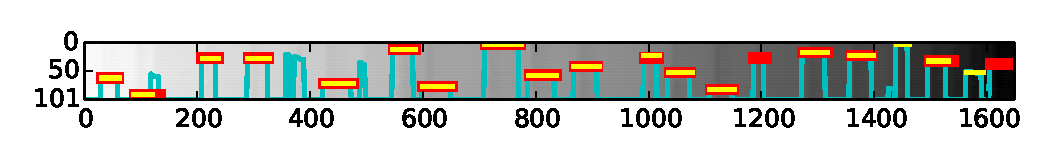
\includegraphics[width=\textwidth]{images/path/Sample0700_sk}
%\vspace*{-3mm}
                \caption{Viterbi decoding from skeleton input.}
                \label{Sample0700_sk}
        \end{subfigure}%
        ~ %add desired spacing between images, e. g. ~, \quad, \qquad, \hfill etc.
          %(or a blank line to force the subfigure onto a new line)

        \begin{subfigure}[c]{0.8\textwidth}
                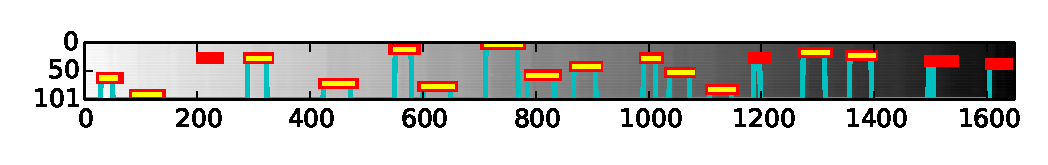
\includegraphics[width=\textwidth]{images/path/Sample0700_cnn}
%\vspace*{-3mm}
                \caption{Viterbi decoding from RGB-D input.}
                \label{Sample0700_cnn}
        \end{subfigure}

        ~ %add desired spacing between images, e. g. ~, \quad, \qquad, \hfill etc.
          %(or a blank line to force the subfigure onto a new line)
        \begin{subfigure}[c]{0.8\textwidth}
                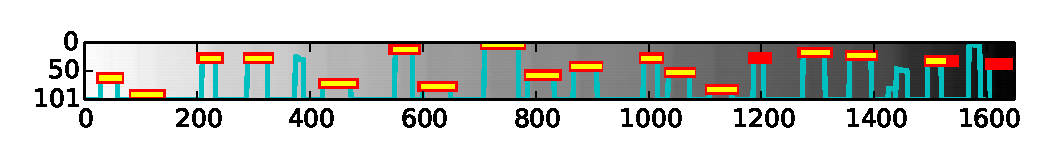
\includegraphics[width=\textwidth]{images/path/Sample0700_combined}
%\vspace*{-3mm}
                \caption{Viterbi decoding from the late fusion of skeleton and RGB-D input.}
                \label{Sample0700_combined}
        \end{subfigure}

  \caption{Viterbi decoding of sample sequence \#700, using skeleton (top), RGB-D (middle) and late fusion system (bottom). The x-axis represents the time and the y-axis represents the hidden states of all the classes and of the ergodic state at the state \emph{101}. Red lines are the ground truth labels, cyan lines represent the viterbi shortest path and yellow lines are the predicted labels. Two modules exhibit complementary behaviors and generally the skeletal module outperforms the depth module. The fusion exploits the complementary properties, \emph{e.g.} around frame 200 the skeleton help solving with the missed detection from the 3DCNN module, while around frame 1450, the 3DCNN module can help suppress the false positive prediction given by skeleton module.
  }\label{fig:Sample0700_comparison}
\end{figure*}

\subsubsection{Tested systems}

We evaluated the recognition performance made by the HMM applied to the emission probabilities estimated from either
the skeleton data, the RGBD image data, the late and early fusion schemes.
%
Note that in all cases the HMM output was further filtered as follows to avoid false alarms.
First, predicted gesture segments of less than 20 frames were considered as noise and discarded.
%
\dwucomline{Actually during the actual test the threshold is set at -inf which does not serve as postprocessing}
In addition, longer but noisy gesture segments whose log-probability (including both emission and transition probabilities)  measured over the viterbi path
was lower than a threshold were discarded.
%
This threshold was set by optimizing the Jaccard index on the validation set  of the training data.


%%%%%%%%%%%%%%%%%%%%%%%%%%%%%%%%%%%%%%%%%%%%%%%%%%%%%%%%%%
 \begin{table}[t]
   \centering
        \begin{tabular}{|l||*{2}{c|}}\hline
            {Module }
            &\makebox[5em]{Validation}&\makebox[5em]{Test}
            \\\hline\hline
            {\small Skeleton -- DBDN }            &  0.783    & 0.779 \\\hline
            {\small RGBD -- 3DCNN }      &  0.752    & 0.717 \\\hline%\hline
            {\small Multimodal Late Fusion }              &  0.817    & 0.809 \\\hline
            {\small Multimodal Early Fusion }             &  0.800    & 0.798 \\\hline
        \end{tabular}
\vspace*{-2mm}
    \caption{Results in terms of Jaccard index \jaccardindex for the different network structures and modalities modeling the emission probabilities.
          }
          \label{Table_score_fusion}
\end{table}
%%%%%%%%%%%%%%%%%%%%%%%%%%%%%%%%%%%%%%%%%%%%%%%%%%%%%%%%%%


%%%%%%%%%%%%%%%%%%%%%%%%%%%%%%%%%%%%%%%%%%%%%%%%%%%%%%%%%%

 \begin{table}[rt]
   \centering
        \begin{tabular}{|ll||*{2}{c|}}\hline
            %\backslashbox{Module}{Evaluation Set}
             &  \% &  \makebox[5em]{Validation}&\makebox[5em]{Test}       \\\hline\hline
            \multirow{2}{*}{Skeleton - DBDN}       & \eventaccuracy                & 86.3     & 83.6 \\
                                            &  \eventconfused           & 11.4     & 12.3 \\
                                            &  \eventmissed           &  2.3     &   4.1 \\\hline\hline
            \multirow{2}{*}{RGB-D - 3DCNN}    & \eventaccuracy              & 78.7     & 75.8  \\
                                            &  \eventconfused           & 5.2     &  4.5 \\
                                            &  \eventmissed           & 16.1     & 19.7  \\\hline\hline
            \multirow{2}{*}{Multimodal Late Fusion}   &  \eventaccuracy    & 87.9     & 86.4 \\
                                                      &  \eventconfused    & 9.1     & 8.7 \\
                                                      &  \eventmissed      & 3.0      & 4.9 \\\hline
           \multirow{2}{*}{Multimodal Early Fusion}   &  \eventaccuracy    & 86.5     & 85.5\\
                                                      &  \eventconfused    & 7.3      & 6.8 \\
                                                      &  \eventmissed      & 6.2      & 7.7 \\\hline
        \end{tabular}
\vspace*{-2mm}
    \caption{
       Gesture classification performance at the event level, in percentage of the number of ground truth gestures.
%\mycomline{table to be finished as for the skeleton}
          }
          \label{tab:eventperformance}
\end{table}

%%%%%%%%%%%%%%%%%%%%%%%%%%%%%%%%%%%%%%%%%%%%%%%%%%%%%%%%%%

\subsection{Results}\label{sec:results}

\mycomline{Confusion matrices are fine. However, would it be possible to know the classifiction accuracy of the different classes, for each modality? (i.e the diagonal elements of the confusion matrix? i.e. for instance to look at lowest/highest results? and it improves with fusion?}

\mypartitle{Overall results.}
%
The overal performance of the algorithms are given in Tables~\ref{Table_score_fusion} and~\ref{tab:eventperformance}.
%
As can be observed, the skeleton module usually  performs better than the RGBD module.
In addition, its generalization capability  is better than that of the RGBD module,
especially when measured with the Jaccard index where there is almost no drop of performance between the validation and test data.
%
One possible explanation is that the information in the skeleton data is more robust, as it benefited from training using huge and highly
varied data~\cite{shotton2011real}: around on million images from both realistic and synthetic depth images were used to train
the decision forest classifiers involved in the joints extraction.
%
On the over hand, as the  RGBD module relies on  the raw data and was learned only from the ChaLearn training set, it may
suffer from some overfitting.
%
Another interesting conclusion that can be drawn from Table~\ref{tab:eventperformance} is that while most errors from the RGB-D module are due to under detection
(the \eventmissed rate is 19.7\%, whereas it is only 4.1\% for the skeleton), the skeleton module is more reactive to gesture activity, but makes more mistakes
(the \eventconfused rate is 12.3\% vs 4.5\% for RGB-D).


Finally, the results also demonstrate  that the combination of both modalities is more robust,
as shown by the recognition rate increase and the smaller drop in the generalization performance
%, both at the \jaccardindex and event level
(for instance the decrease of the \eventaccuracy rate is lower than for the skeleton data alone).



%%%%%%%%%%%%%%%%%%%%%%%%%%%%%%%%%%%%%%%%%%%%%%%%%%%%%%%%%%
\begin{figure}[t]
        \centering
        \begin{subfigure}[c]{.36\textwidth}
                \includegraphics[width=\textwidth]{images/cm/cm_sk}
\vspace*{-3mm}
                \caption{Skeleton - DBDN}
                \label{sk_cm}
        \end{subfigure}%
        ~ %add desired spacing between images, e. g. ~, \quad, \qquad, \hfill etc.
          %(or a blank line to force the subfigure onto a new line)

        \begin{subfigure}[c]{0.36\textwidth}
                \includegraphics[width=\textwidth]{images/cm/cm_cnn}
\vspace*{-3mm}
                \caption{RGBD - 3DCNN}
                \label{cnn_cm}
        \end{subfigure}

        ~ %add desired spacing between images, e. g. ~, \quad, \qquad, \hfill etc.
          %(or a blank line to force the subfigure onto a new line)
        \begin{subfigure}[c]{0.36\textwidth}
                \includegraphics[width=\textwidth]{images/cm/cm_combination}
\vspace*{-3mm}
                \caption{Multimodal Late Fusion}
                \label{fusion_cm}
        \end{subfigure}

  \caption{Confusion Matrices  for the different modalities.}
\label{fig:confusion_matrix}
\end{figure}
%%%%%%%%%%%%%%%%%%%%%%%%%%%%%%%%%%%%%%%%%%%%%%%%%%%%%%%%%%

\mypartitle{Confusion matrices.}
%
The confusion matrices in Fig.~\ref{fig:confusion_matrix} better illustrate the complementarity of the behaviors of the two modalities.
%
The higher underdetection of RGB-D is clearly visible (whiter matrix, except last 'undetected' column).
%

We can also notice that some gestures are more easily recognized than others,
or catch the difficult instances of other gestures.
This is the case for instance of the ``Basta" gesture,
whose arms motion  resembles the  start and end of the arm motion of many other gestures (see Fig.~\ref{fig:chalearnclasses}).
Whatever the modality, it thus tends to be over-detected for all gesture classes, whenever the
likelihood of the instances are low when being evaluated using the HMM states associated with their true label
due to too much variability.
%
Similarly, the hand movement and pose of the ``Buenissimo" gesture is present in several other gesture classes,
whose instances are then often confused with ``Buenissimo" when relying on the skeleton information alone.
%
However, as these gestures differ primarily in their hand pose, such confusion is much more reduced using the RGB-D domain,
or when fusing  the skeleton and RGB-D modules.
%
The complementary properties of the two modalities is also illustrated from the Viterbi path decoding plot in Fig.~\ref{fig:Sample0700_comparison}.
In general, the benefit of this complementarity in the fusion between arm pose/gesture and hand pose
can be observed from the whiter confusion matrix than in the skeleton case (less confusion due to hand pose information from RGB-D)
and much less under-detection than in the RGB-D case (better upper-body pose discrimination thanks to skeleton input).
%

However, the modalities by themselves have more difficulties to correct the recognition errors which are due to variations coming from the performer,
like differentiating  people that gesticulate more, as illustrated in Fig.~\ref{fig:bodydynamics}.

\mypartitle{Late vs. Early fusion.}



We compare the results of late fusion and early fusion in Tab.~\ref{Table_score_fusion} and we can see that the early fusion system didn't outperform the late fusion system. The result is counter-intuitive because we expect the early fusion  multimodal feature learning will extract semantically meaningful shared representations, outperforming individual modalities, and the early fusion scheme�s efficacy against the traditional method of late fusion. One possible explanation could be that one individual module has dominant effect on the learning process so as to skew the network towards learning that specific module. The mean activations of the neurons for each modules in Fig.~\ref{fig:fusion} indicate the aforementioned conjecture.
 The mean activation of skeleton module neurons is predominantly larger than the RGBD ConvNet's (0.57 \emph{vs.} 0.056). Though that skeleton module has logistic units whereas ConvNet module has relu unit~\cite{DBLP:journals/corr/PigouODHD15}, the mean activations of the two are not directly comparable. However, 10 times the difference of mean activation indicates the bias during the multimodal fine-tuning phase that could cause the less than expected performance.

\mycomline{In this comment on the results and benefit of the temporal model, as we discussed.}
%

\mypartitle{HMM benefit.}


\mypartitle{Comparison with the state-of-the-art. In particular, add discussion that other temporal module could be used,
including those that could lead to the training of a full deep-neural network.  }
%

To investigate the benefit of temporal modelling of the proposed system, we compare the model that discards temporal modelling. Specially, once, we collect the emission probability \emissionprob{}, we average the hidden states for each gesture class and obtain the frame based gesture class prediction \gestureEmissionProb where \gesturehiddenstateFrame denotes the gesture variables. After temporal smoothing for each frame, a threshold for cutting the begin and end of active gesture is chosen by a validation set.

\dwucomline{A new Fig. will be included}
The performance of recent state-of-the-art techniques is given in Table~\ref{tab:soa}.

\mycomline{Distinguish handcrafted features and neural net approaches. explain the differences in models that potentially lead to the difference.}


%%%%%%%%%%%%%%%%%%%%%%%%%%%%%%%%%%%%%%%%%%%%%%%%%%%%%%%%%%

\begin{figure}[tb]
        \centering

        \begin{subfigure}[c]{.2\textwidth}
        \centering
                \includegraphics[width=3cm,height=3cm, trim=120 100 100 50, clip]{images/good}
      \vspace*{-2mm}
                \caption{Well-recognised}
        \end{subfigure}%
        %
        \begin{subfigure}[c]{0.2\textwidth}
        \centering
                \includegraphics[width=3cm,height=3cm, trim=120 100 100 50, clip]{images/bad}
      \vspace*{-2mm}
                \caption{Poorly-recognised}
        \end{subfigure}
      \vspace*{-3mm}
  \caption{
\mycomline{Show more sample to illustrate the dynamic - would be good to show the instances for the same gestures - the jaccard index below are obtained using which module?}
Examples of performer variations in the  upper body dynamic.
While most performers tend to keep their upper-body static while performing the gesture leading to good recognition performance (left, Jaccard index of 0.94),
others vehemently move their body when doing the gestures, making them harder to recognize (right, Jaccard index of 0.34).
}
\label{fig:bodydynamics}
\end{figure}



%%%%%%%%%%%%%%%%%%%%%%%%%%%%%%%%%%%%%%%%%%%%%%%%%%%%%%%%%%%%
 \begin{table}[t]
   \centering
        \begin{tabular}{|l||*{3}{c|}}\hline
            {Module}
            &\makebox[3em]{Skeleton}&\makebox[6em]{RGBD}&\makebox[3em]{Fusion}
            \\\hline\hline
            {~\cite{neverova2014multi}} Deep Learning (Step 4)                  &   0.7891     &  0.7990      & \textbf{0.8449}\\\hline
            {~\cite{neverova2014multi}} Deep Learning (multiscal)               &   0.8080     &  0.8096      & \textbf{ 0.8488}\\\hline
            {~\cite{Monnier2014multi}} 3 Set Skeletal \& HOG                   &   0.791     & -           & 0.8220 \\\hline
            {~\cite{Chang2014multi}}   Handcrafted features                       &  \textbf{0.7948}     & -           & 0.8268\\\hline
            {~\cite{Peng2014multi}}    Dense Trajectory                         &  -          & \textbf{0.7919}      & -\\\hline
            {~\cite{lio2014deep}}      CNN                                      &  -          & 0.7888      & -\\\hline
            {~\cite{wu2014deep}}    Deep Learning                               &  0.7468     & 0.6371      & 0.8045\\\hline \hline
            \textbf{\emph{DDNN}} (this work)                                    &  0.7792    & 0.7168  & 0.8091\\\hline
        \end{tabular}
    \caption{
\mycomline{Add one or two worse results; separate hand crafted features from neural net methods.}
    Comparison of results in terms of the ChaLearn Jaccard index with state-of-the-art related works.
          }
          \label{tab:soa}
\end{table}


\subsection{Computational Complexity}
\label{sec:ComputationalComplexity}

We can distinguish between two complexity: the training one, and the test one.

\mycomline{Say a few words about the training complexity (which part takes longer -skeleton ? RGBD? - and how long does it take on the Chalearn dataset.}

\mypartitle{Complexity at training time.}
Although training the deep neural network using stochastic gradient descent is computationally intensive, the reuse of our pre-train network parameters could help with the better initialisation of the fusion network and fast convergence. Different modality training time also varies. Specifically, the training time of each epoch for DBN skeleton module is less than 300 second and allowing training 500 epochs within 2 days. The training time of each epoch for 3DCNN of RGB-D  module is much computational expensive, taking more than 10,000 second. Hence, 40 epochs takes around 5 days to train.

\mypartitle{Complexity at test time.}
%
Given the learned models,  our framework can perform real-time video sequence labelling with a low inference cost.
%
More specifically, a single feed forward neural network incurs linear computational time ($\mathcal{O}(T)$),
and is efficient because it requires only matrix products and convolution operations.
The complexity of the Viterbi algorithm is itself of $\mathcal{O} (T* |S|^2)$, where
$T$ is the number of frames and $|S|$ the number of states, and thus performs real-timegiven our state-space.

In practice, using a modern GPU (GeForece GTX TITAN Black), our multimodal neural network can be deployed at 90 FPS using the
Theano library~\cite{Bastien-Theano-2012}.
The preprocessing part takes most of the time and our un-optimized version runs at 25 FPS, while the
 Viterbi decoding  runs at 90 FPS. Hence, the overall system can achieve faster than real-time performance.





\endinput
